% answers.tex —— 2001 年·春季上海卷 · 参考答案与详细解析片段
% 由 tools/generate_projects.py 依来源总账自 2001/2001_数学真题_春季上海_试题.md + 2001/2001_数学真题_春季上海_解析正文.md + 2001/2001_数学真题_春季上海_答案要点.md 生成，勿手改（改源 MD 后重跑）


\begin{gktip}
固定源 PDF 为印刷页码 83–84 的两页题面，不附答案。以下解析均依据题面独立复算；第 19、20 题的图形在 LaTeX 工程中以 TikZ/PGFPlots 矢量源重绘。
\end{gktip}

\gkpart{一、填空题}

\begin{answer}
\gksolhead{1}{}

\textbf{题目}：

函数 $f(x)=x^2+1$（$x\le0$）的反函数 $f^{-1}(x)=$\gkblank{}。

\Needspace{4\baselineskip}
\textbf{解析}

\Needspace{5\baselineskip}
令 $y=x^2+1$，且 $x\le0$。由 $x^2=y-1$ 及 $x\le0$，得

\nopagebreak[4]
\[
x=-\sqrt{y-1}
\]

\Needspace{5\baselineskip}
原函数的值域为 $[1,+\infty)$，所以

\nopagebreak[4]
\[
f^{-1}(x)=-\sqrt{x-1},\qquad x\ge1
\]

\gkanswer{答案：$f^{-1}(x)=-\sqrt{x-1}$（$x\ge1$）。}

\end{answer}
\begin{answer}
\gksolhead{2}{}

\textbf{题目}：

若复数 $z$ 满足方程 $zi=i-1$（$i$ 是虚数单位），则 $z=$\gkblank{}。

\Needspace{4\baselineskip}
\textbf{解析}

\Needspace{5\baselineskip}
由 $zi=i-1$，两边同除以 $i$，得

\nopagebreak[4]
\[
z=\frac{i-1}{i}=1+i
\]

\gkanswer{答案：$z=1+i$。}

\end{answer}
\begin{answer}
\gksolhead{3}{}

\textbf{题目}：

\Needspace{5\baselineskip}
函数

\nopagebreak[4]
\[
y=\dfrac{\sin x}{1-\cos x}
\]

的最小正周期为\gkblank{}。

\Needspace{4\baselineskip}
\textbf{解析}

\Needspace{5\baselineskip}
在函数有定义时，

\nopagebreak[4]
\[
\frac{\sin x}{1-\cos x}
=\frac{2\sin\frac{x}{2}\cos\frac{x}{2}}{2\sin^2\frac{x}{2}}
=\cot\frac{x}{2}
\]

\Needspace{5\baselineskip}
函数 $\cot u$ 的最小正周期为 $\pi$，因此原函数的最小正周期为

\nopagebreak[4]
\[
2\pi
\]

\gkanswer{答案：$2\pi$。}

\end{answer}
\begin{answer}
\gksolhead{4}{}

\textbf{题目}：

\Needspace{5\baselineskip}
二项式

\nopagebreak[4]
\[
\left(x+\dfrac1x\right)^6
\]

的展开式中常数项的值为\gkblank{}。

\Needspace{4\baselineskip}
\textbf{解析}

\Needspace{5\baselineskip}
展开式的一般项为

\nopagebreak[4]
\[
\binom6r x^{6-r}\left(\frac1x\right)^r
=\binom6r x^{6-2r}
\]

\Needspace{5\baselineskip}
常数项要求 $6-2r=0$，即 $r=3$，所以常数项为

\nopagebreak[4]
\[
\binom63=20
\]

\gkanswer{答案：$20$。}

\end{answer}
\begin{answer}
\gksolhead{5}{}

\textbf{题目}：

若双曲线的一个顶点坐标为 $(3,0)$，焦距为 $10$，则它的标准方程为\gkblank{}。

\Needspace{4\baselineskip}
\textbf{解析}

\Needspace{5\baselineskip}
由顶点坐标可知双曲线的实半轴 $a=3$。焦距为 $10$，故 $2c=10$，即 $c=5$。于是

\nopagebreak[4]
\[
b^2=c^2-a^2=25-9=16
\]

\Needspace{5\baselineskip}
所以标准方程为

\nopagebreak[4]
\[
\frac{x^2}{9}-\frac{y^2}{16}=1
\]

\gkanswer{答案：$\dfrac{x^2}{9}-\dfrac{y^2}{16}=1$。}

\end{answer}
\begin{answer}
\gksolhead{6}{}

\textbf{题目}：

圆心在直线 $y=x$ 上且与 $x$ 轴相切于点 $(1,0)$ 的圆的方程为\gkblank{}。

\Needspace{4\baselineskip}
\textbf{解析}

\Needspace{5\baselineskip}
圆与 $x$ 轴相切于 $(1,0)$，所以圆心的横坐标为 $1$。又圆心在 $y=x$ 上，圆心为 $(1,1)$，半径为 $1$。因此圆的方程为

\nopagebreak[4]
\[
(x-1)^2+(y-1)^2=1
\]

\gkanswer{答案：$(x-1)^2+(y-1)^2=1$。}

\end{answer}
\begin{answer}
\gksolhead{7}{}

\textbf{题目}：

\Needspace{5\baselineskip}
计算

\nopagebreak[4]
\[
\lim_{n\to\infty}\left(\dfrac{n+3}{n+1}\right)^n
\]

。

\Needspace{4\baselineskip}
\textbf{解析}

\Needspace{5\baselineskip}
有

\nopagebreak[4]
\[
\left(\frac{n+3}{n+1}\right)^n
=\left(1+\frac2{n+1}\right)^n
\]

\Needspace{5\baselineskip}
由基本极限 $\displaystyle\lim_{n\to\infty}\left(1+\frac2n\right)^n=e^2$，可得

\nopagebreak[4]
\[
\lim_{n\to\infty}\left(\frac{n+3}{n+1}\right)^n=e^2
\]

\gkanswer{答案：$e^2$。}

\end{answer}
\begin{answer}
\gksolhead{8}{}

\textbf{题目}：

若向量 $\boldsymbol{\alpha}$、$\boldsymbol{\beta}$ 满足 $\lvert\boldsymbol{\alpha}+\boldsymbol{\beta}\rvert=\lvert\boldsymbol{\alpha}-\boldsymbol{\beta}\rvert$，则 $\boldsymbol{\alpha}$ 与 $\boldsymbol{\beta}$ 所成角的大小为\gkblank{}。

\Needspace{4\baselineskip}
\textbf{解析}

\Needspace{5\baselineskip}
两边平方并展开：

\nopagebreak[4]
\[
\lvert\boldsymbol{\alpha}+\boldsymbol{\beta}\rvert^2
=\lvert\boldsymbol{\alpha}\rvert^2
+2\boldsymbol{\alpha}\cdot\boldsymbol{\beta}
+\lvert\boldsymbol{\beta}\rvert^2
\]

\nopagebreak[4]
\[
\lvert\boldsymbol{\alpha}-\boldsymbol{\beta}\rvert^2
=\lvert\boldsymbol{\alpha}\rvert^2
-2\boldsymbol{\alpha}\cdot\boldsymbol{\beta}
+\lvert\boldsymbol{\beta}\rvert^2
\]

题设等式给出 $\boldsymbol{\alpha}\cdot\boldsymbol{\beta}=0$，所以两向量垂直，所成角为 $90^\circ$。

\gkanswer{答案：$90^\circ$。}

\end{answer}
\begin{answer}
\gksolhead{9}{}

\textbf{题目}：

在大小相同的 $6$ 个球中，$2$ 个红球，$4$ 个是白球。若从中任意选取 $3$ 个，则所选的 $3$ 个球中至少有 $1$ 个红球的概率是\gkblank{}。（结果用分数表示）

\Needspace{4\baselineskip}
\textbf{解析}

\Needspace{5\baselineskip}
从 $6$ 个球中任选 $3$ 个共有 $\binom63$ 种选法。所选的 $3$ 个球中至少有 $1$ 个红球的对立事件是全为白球，故所求概率为

\nopagebreak[4]
\[
1-\frac{\binom43}{\binom63}
=1-\frac4{20}
=\frac45
\]

\gkanswer{答案：$\dfrac45$。}

\end{answer}
\begin{answer}
\gksolhead{10}{}

\textbf{题目}：

\Needspace{5\baselineskip}
若记号“$\ast$”表示求两个实数 $a$ 与 $b$ 的算术平均数的运算，即

\nopagebreak[4]
\[
a\ast b=\dfrac{a+b}{2}
\]

则两边均含有运算符号“$\ast$”和“$+$”，且对于任意 $3$ 个实数 $a\text{、}b\text{、}c$ 都能成立的一个等式可以是\gkblank{}。

\Needspace{4\baselineskip}
\textbf{解析}

\Needspace{5\baselineskip}
运算 $\ast$ 表示算术平均数，因此满足交换律

\nopagebreak[4]
\[
a\ast b=b\ast a
\]

\Needspace{5\baselineskip}
两边同加 $c$，便得到一个符合题意的等式

\nopagebreak[4]
\[
a\ast b+c=b\ast a+c
\]

\gkanswer{答案：$a\ast b+c=b\ast a+c$。}

\end{answer}
\begin{answer}
\gksolhead{11}{}

\textbf{题目}：

关于 $x$ 的函数 $f(x)=\sin(x+\varphi)$ 有以下命题：

（1）对任意的 $\varphi$，$f(x)$ 都是非奇非偶函数；

（2）不存在 $\varphi$，使 $f(x)$ 既是奇函数，又是偶函数；

（3）存在 $\varphi$，使 $f(x)$ 是奇函数；

（4）对任意的 $\varphi$，$f(x)$ 都不是偶函数。

其中一个假命题的序号是\gkblank{}。因为当 $\varphi=$\gkblank{} 时，该命题的结论不成立。

\Needspace{4\baselineskip}
\textbf{解析}

当 $\varphi=0$ 时，$f(x)=\sin x$ 是奇函数，所以命题（1）“对任意的 $\varphi$，$f(x)$ 都是非奇非偶函数”不成立。因此可填序号①和 $\varphi=0$。

题目只要求填写一个假命题。事实上，当 $\varphi=\dfrac\pi2$ 时，$f(x)=\cos x$ 是偶函数，命题（4）也不成立。

命题（2）成立，因为一个同时为奇函数和偶函数的函数必须恒为零，而 $\sin(x+\varphi)$ 不可能恒为零；命题（3）也成立，例如 $\varphi=0$ 时函数为奇函数。

\gkanswer{答案：①，$0$（也可填④，$\dfrac\pi2$）。}

\end{answer}
\begin{answer}
\gksolhead{12}{}

\textbf{题目}：

甲、乙两人于同一天分别携款 $1$ 万元到银行储蓄，甲存五年期定期储蓄，年利率为 $2.88\%$。乙存一年期定期储蓄，年利率为 $2.25\%$，并在每年到期时将本息续存一年期定期储蓄。按规定每次计息时，储户须交纳利息的 $20\%$ 作为利息税。若存满五年后两人同时从银行取出存款，则甲与乙所得本息之和的差为\gkblank{}元。（假定利率五年内保持不变，结果精确到 $1$ 分）

\Needspace{4\baselineskip}
\textbf{解析}

\Needspace{5\baselineskip}
甲的五年期储蓄在五年后所得本息为

\nopagebreak[4]
\[
10000\left(1+5\times2.88\%\times(1-20\%)\right)
=11152
\]

\Needspace{5\baselineskip}
乙每年计息并续存，扣税后的年增长因子为

\nopagebreak[4]
\[
1+2.25\%\times(1-20\%)=1.018
\]

\Needspace{5\baselineskip}
五年后乙所得本息为

\nopagebreak[4]
\[
10000(1.018)^5=10932.98846769568
\]

\Needspace{5\baselineskip}
所以甲与乙所得本息之和的差为

\nopagebreak[4]
\[
11152-10932.98846769568=219.01153230432
\]

精确到 $1$ 分为 $219.01$ 元。

\gkanswer{答案：$219.01$ 元，甲比乙多。}

\end{answer}
\gkpart{二、选择题}

\begin{answer}
\gksolhead{13}{}

\textbf{题目}：

若 $a\text{、}b$ 为实数，则 $a>b>0$ 是 $a^2>b^2$ 的\mbox{（　　）}

（A）充分不必要条件　　（B）必要不充分条件

（C）充要条件　　（D）既非充分条件也非必要条件

\Needspace{4\baselineskip}
\textbf{解析}

\Needspace{5\baselineskip}
若 $a>b>0$，则

\nopagebreak[4]
\[
a^2-b^2=(a-b)(a+b)>0
\]

反过来，若 $a^2>b^2$ 且 $a\text{、}b$ 均为正数，则 $a>b$。所以 $a>b>0$ 是 $a^2>b^2$ 的充要条件，选 C。

\gkanswer{答案：C。}

\end{answer}
\begin{answer}
\gksolhead{14}{}

\textbf{题目}：

若直线 $x=1$ 的倾斜角为 $\alpha$，则 $\alpha$\mbox{（　　）}

（A）等于 $0$　　（B）等于 $\dfrac\pi4$　　（C）等于 $\dfrac\pi2$　　（D）不存在

\Needspace{4\baselineskip}
\textbf{解析}

\Needspace{5\baselineskip}
直线的倾斜角取值范围为 $[0,\pi)$。直线 $x=1$ 是竖直直线，其倾斜角为

\nopagebreak[4]
\[
\alpha=\frac\pi2
\]

选 C。

\gkanswer{答案：C。}

\end{answer}
\begin{answer}
\gksolhead{15}{}

\textbf{题目}：

若有平面 $\alpha$ 与 $\beta$，且 $\alpha\cap\beta=l$，$\alpha\perp\beta$，$P\in\alpha$，$P\notin l$，则下列命题中的假命题为\mbox{（　　）}

（A）过点 $P$ 且垂直于 $\alpha$ 的直线平行于 $\beta$

（B）过点 $P$ 且垂直于 $l$ 的平面垂直于 $\beta$

（C）过点 $P$ 且垂直于 $\beta$ 的直线在 $\alpha$ 内

（D）过点 $P$ 且垂直于 $l$ 的直线在 $\alpha$ 内

\Needspace{4\baselineskip}
\textbf{解析}

在两个互相垂直的平面中，垂直于一个平面的直线方向平行于另一个平面，所以（A）正确；过 $P$ 且垂直于交线 $l$ 的平面垂直于含有 $l$ 的平面 $\beta$，所以（B）正确；过 $P$ 且垂直于 $\beta$ 的直线方向在 $\alpha$ 内，所以（C）正确。

（D）不成立。取 $\alpha$ 为 $xOy$ 平面，$\beta$ 为 $xOz$ 平面，交线为 $x$ 轴，取 $P=(0,1,0)$。过 $P$ 且沿 $z$ 轴方向的直线垂直于 $l$，但不在 $\alpha$ 内。因此假命题为（D），选 D。

\gkanswer{答案：D。}

\end{answer}
\begin{answer}
\gksolhead{16}{}

\textbf{题目}：

若数列 $\{a_n\}$ 前 $8$ 项的值各异，且 $a_{n+8}=a_n$ 对任意的 $n\in\mathbb N$ 都成立，则下列数列中可取遍 $\{a_n\}$ 前 $8$ 项值的数列为\mbox{（　　）}

（A）$\{a_{2k+1}\}$　　（B）$\{a_{3k+1}\}$　　（C）$\{a_{4k+1}\}$　　（D）$\{a_{6k+1}\}$

\Needspace{4\baselineskip}
\textbf{解析}

由于 $a_{n+8}=a_n$ 且前 $8$ 项互不相同，题目等价于考察下标对 $8$ 的余数。

对 $\{a_{3k+1}\}$，因为 $\gcd(3,8)=1$，当 $k$ 连续取值时，$3k+1$ 模 $8$ 的余数可以遍历全部 $8$ 个余数。因此它可以取遍前 $8$ 项的值。其他选项的步长与 $8$ 的最大公因数不为 $1$，只能取到部分余数，故选 B。

\gkanswer{答案：B。}

\end{answer}
\gkpart{三、解答题}

\begin{answer}
\gksolhead{17}{}

\textbf{题目}：

\Needspace{5\baselineskip}
已知 $\mathbb R$ 为全集，

\nopagebreak[4]
\[
A=\left\{x\mid\log_{\frac12}(3-x)\ge-2\right\},\qquad
B=\left\{x\mid\dfrac5{x+2}\ge1\right\}
\]

求 $\overline A\cap B$。

\Needspace{4\baselineskip}
\textbf{解析}

\Needspace{5\baselineskip}
对 $A$，先由真数条件得 $3-x>0$，即 $x<3$。由于底数 $\dfrac12$ 小于 $1$，对数函数递减，所以

\nopagebreak[4]
\[
\log_{\frac12}(3-x)\ge-2
\Longleftrightarrow
0<3-x\le\left(\frac12\right)^{-2}=4
\]

\Needspace{5\baselineskip}
从而

\nopagebreak[4]
\[
A=[-1,3)
\]

\Needspace{5\baselineskip}
对 $B$，$x\ne-2$，且

\nopagebreak[4]
\[
\frac5{x+2}\ge1
\Longleftrightarrow
\frac{3-x}{x+2}\ge0
\]

\Needspace{5\baselineskip}
作符号分析得

\nopagebreak[4]
\[
B=(-2,3]
\]

\Needspace{5\baselineskip}
因此

\nopagebreak[4]
\[
\overline A\cap B
=\left((-\infty,-1)\cup[3,+\infty)\right)\cap(-2,3]
=(-2,-1)\cup\{3\}
\]

\gkanswer{答案：$\left(-2,-1\right)\cup\{3\}$。}

\end{answer}
\begin{answer}
\gksolhead{18}{}

\textbf{题目}：

\Needspace{5\baselineskip}
已知

\nopagebreak[4]
\[
\dfrac{2\sin^2\alpha+\sin2\alpha}{1+\tan\alpha}=k
\quad\left(\dfrac\pi4<\alpha<\dfrac\pi2\right)
\]

试用 $k$ 表示 $\sin\alpha-\cos\alpha$ 的值。

\Needspace{4\baselineskip}
\textbf{解析}

\Needspace{5\baselineskip}
由 $\dfrac\pi4<\alpha<\dfrac\pi2$，分母不为零，且

\nopagebreak[4]
\[
\frac{2\sin^2\alpha+\sin2\alpha}{1+\tan\alpha}
=\frac{2\sin^2\alpha+2\sin\alpha\cos\alpha}{1+\frac{\sin\alpha}{\cos\alpha}}
=\frac{2\sin\alpha(\sin\alpha+\cos\alpha)}
{\frac{\sin\alpha+\cos\alpha}{\cos\alpha}}
=2\sin\alpha\cos\alpha
=\sin2\alpha
\]

\Needspace{5\baselineskip}
所以 $k=\sin2\alpha$。又因 $\alpha>\dfrac\pi4$，有 $\sin\alpha-\cos\alpha>0$，于是

\nopagebreak[4]
\[
(\sin\alpha-\cos\alpha)^2
=\sin^2\alpha+\cos^2\alpha-2\sin\alpha\cos\alpha
=1-k
\]

\Needspace{5\baselineskip}
故

\nopagebreak[4]
\[
\sin\alpha-\cos\alpha=\sqrt{1-k}
\]

\gkanswer{答案：$\sqrt{1-k}$。}

\end{answer}
\begin{answer}
\gksolhead{19}{}

\textbf{题目}：

用一块钢锭浇铸一个厚度均匀，且全面积为 $2$ 平方米的正四棱锥形有盖容器（如图），设容器的高为 $h$ 米，盖子边长为 $a$ 米。
\nopagebreak[4]
\begin{center}% 2001 年春季上海卷第 19 题：正四棱锥形有盖容器
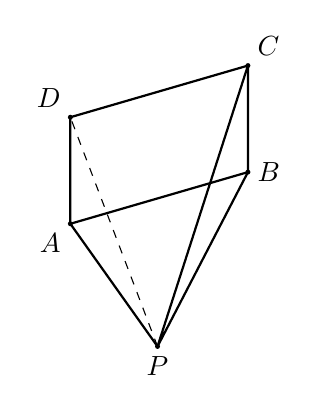
\begin{tikzpicture}[>=stealth, scale=0.82]
  \coordinate (A) at (0,0);
  \coordinate (B) at (2.75,0.8);
  \coordinate (C) at (2.75,2.45);
  \coordinate (D) at (0,1.65);
  \coordinate (P) at (1.35,-1.9);

  \draw[thick] (A)--(B)--(C)--(D)--cycle;
  \draw[thick] (P)--(A) (P)--(B) (P)--(C);
  \draw[dashed] (P)--(D);

  \fill (A) circle (1.1pt) node[below left] {$A$};
  \fill (B) circle (1.1pt) node[right] {$B$};
  \fill (C) circle (1.1pt) node[above right] {$C$};
  \fill (D) circle (1.1pt) node[above left] {$D$};
  \fill (P) circle (1.1pt) node[below] {$P$};
\end{tikzpicture}
\end{center}
\nopagebreak[4]
（1） 求 $a$ 关于 $h$ 的函数解析式；

（2） 设容器的容积为 $V$ 立方米，则当 $h$ 为何值时，$V$ 最大？求出 $V$ 的最大值。

注：求解本题时，不计容器的厚度。

\Needspace{4\baselineskip}
\textbf{解析}

\gksubpart{(1)}

\Needspace{5\baselineskip}
设正四棱锥侧面的斜高为 $l$。由正四棱锥的高和盖子边长，得

\nopagebreak[4]
\[
l=\sqrt{h^2+\left(\frac a2\right)^2}
\]

\Needspace{5\baselineskip}
容器的全面积由盖子的正方形和四个全等的三角形侧面组成，因此

\nopagebreak[4]
\[
a^2+4\cdot\frac12al=2
\]

\Needspace{5\baselineskip}
即

\nopagebreak[4]
\[
a^2+2a\sqrt{h^2+\frac{a^2}{4}}=2
\]

\Needspace{5\baselineskip}
因 $a>0$，可将根式项移项后平方：

\nopagebreak[4]
\[
(2-a^2)^2
=4a^2\left(h^2+\frac{a^2}{4}\right)
\]

\Needspace{5\baselineskip}
化简得

\nopagebreak[4]
\[
4-4a^2=4a^2h^2
\]

\Needspace{5\baselineskip}
所以

\nopagebreak[4]
\[
a^2(1+h^2)=1
\]

\Needspace{5\baselineskip}
从而

\nopagebreak[4]
\[
a=\frac1{\sqrt{1+h^2}},\qquad h>0
\]

\gksubpart{(2)}

\Needspace{5\baselineskip}
容器的容积为

\nopagebreak[4]
\[
V=\frac13a^2h
=\frac{h}{3(1+h^2)}
\]

\Needspace{5\baselineskip}
求导得

\nopagebreak[4]
\[
V'(h)=\frac{1-h^2}{3(1+h^2)^2}
\]

\Needspace{5\baselineskip}
故 $V$ 在 $0<h<1$ 时递增，在 $h>1$ 时递减。当 $h=1$ 时取得最大值，此时

\nopagebreak[4]
\[
V_{\max}=\frac1{3(1+1)}=\frac16
\]

\gkanswer{答案（1）：$a=\dfrac1{\sqrt{1+h^2}}$。}

\gkanswer{答案（2）：$h=1$ 时 $V$ 最大，最大值为 $\dfrac16$ 立方米。}

\end{answer}
\begin{answer}
\gksolhead{20}{}

\textbf{题目}：

在长方体 $ABCD-A_1B_1C_1D_1$ 中，点 $E\text{、}F$ 分别在 $BB_1\text{、}DD_1$ 上，且 $AE\perp A_1B$，$AF\perp A_1D$。
\nopagebreak[4]
\begin{center}% 2001 年春季上海卷第 20 题：长方体中的点与平面
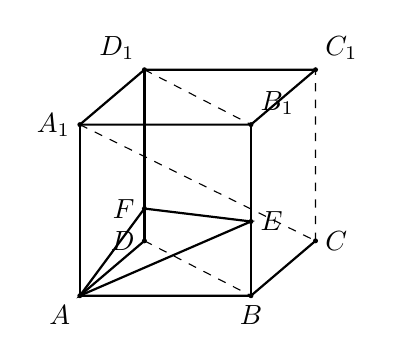
\begin{tikzpicture}[>=stealth, scale=0.82]
  \coordinate (A) at (0,0);
  \coordinate (B) at (2.65,0);
  \coordinate (C) at (3.65,0.85);
  \coordinate (D) at (1,0.85);
  \coordinate (A1) at (0,2.65);
  \coordinate (B1) at (2.65,2.65);
  \coordinate (C1) at (3.65,3.5);
  \coordinate (D1) at (1,3.5);
  \coordinate (E) at (2.65,1.15);
  \coordinate (F) at (1,1.35);

  \draw[thick] (A)--(B)--(C);
  \draw[thick] (A)--(D);
  \draw[thick] (A1)--(B1)--(C1);
  \draw[thick] (A1)--(D1)--(C1);
  \draw[thick] (A)--(A1) (B)--(B1) (D)--(D1);
  \draw[dashed] (C)--(C1) (D1)--(B1) (D)--(B);
  \draw[thick] (A)--(E)--(F)--cycle;
  \draw[dashed] (A1)--(C);

  \fill (A) circle (1.1pt) node[below left] {$A$};
  \fill (B) circle (1.1pt) node[below] {$B$};
  \fill (C) circle (1.1pt) node[right] {$C$};
  \fill (D) circle (1.1pt) node[left] {$D$};
  \fill (A1) circle (1.1pt) node[left] {$A_1$};
  \fill (B1) circle (1.1pt) node[above right] {$B_1$};
  \fill (C1) circle (1.1pt) node[above right] {$C_1$};
  \fill (D1) circle (1.1pt) node[above left] {$D_1$};
  \fill (E) circle (1.1pt) node[right] {$E$};
  \fill (F) circle (1.1pt) node[left] {$F$};
\end{tikzpicture}
\end{center}
\nopagebreak[4]
（1） 求证：$A_1C\perp$ 平面 $AEF$；

（2） 若规定两个平面所成的角是这两个平面所组成的二面角中的锐角（或直角），则在空间中有定理：若两条直线分别垂直于两个平面，则这两条直线所成的角与这两个平面所成的角相等。试根据上述定理，在 $AB=4$，$AD=3$，$AA_1=5$ 时，求平面 $AEF$ 与平面 $D_1B_1BD$ 所成的角的大小。（用反三角函数值表示）

\Needspace{4\baselineskip}
\textbf{解析}

\gksubpart{(1)}

\Needspace{5\baselineskip}
建立空间直角坐标系，令

\nopagebreak[4]
\[
A=(0,0,0),\quad B=(p,0,0),\quad D=(0,q,0),\quad A_1=(0,0,r)
\]

\Needspace{5\baselineskip}
则 $C=(p,q,0)$。设 $E=(p,0,u)$，$F=(0,q,v)$。由题设的垂直关系，

\nopagebreak[4]
\[
\overrightarrow{AE}\cdot\overrightarrow{A_1B}
=(p,0,u)\cdot(p,0,-r)
=p^2-ru=0
\]

\nopagebreak[4]
\[
\overrightarrow{AF}\cdot\overrightarrow{A_1D}
=(0,q,v)\cdot(0,q,-r)
=q^2-rv=0
\]

\Needspace{5\baselineskip}
因此 $u=\dfrac{p^2}{r}$，$v=\dfrac{q^2}{r}$。又

\nopagebreak[4]
\[
\overrightarrow{A_1C}=(p,q,-r)
\]

\Needspace{5\baselineskip}
所以

\nopagebreak[4]
\[
\overrightarrow{A_1C}\cdot\overrightarrow{AE}
=(p,q,-r)\cdot\left(p,0,\frac{p^2}{r}\right)=0
\]

\Needspace{5\baselineskip}
以及

\nopagebreak[4]
\[
\overrightarrow{A_1C}\cdot\overrightarrow{AF}
=(p,q,-r)\cdot\left(0,q,\frac{q^2}{r}\right)=0
\]

向量 $\overrightarrow{AE}$、$\overrightarrow{AF}$ 是平面 $AEF$ 内两条相交直线，所以 $A_1C\perp$ 平面 $AEF$。

\gksubpart{(2)}

\Needspace{5\baselineskip}
当 $AB=4$，$AD=3$，$AA_1=5$ 时，

\nopagebreak[4]
\[
\overrightarrow{A_1C}=(4,3,-5)
\]

\Needspace{5\baselineskip}
它是平面 $AEF$ 的法向量。平面 $D_1B_1BD$ 内的两条相交直线可取 $BD$ 和 $BB_1$，故该平面的法向量可取

\nopagebreak[4]
\[
\overrightarrow{BD}\times\overrightarrow{BB_1}
=(-4,3,0)\times(0,0,5)
=(15,20,0)
\sim(3,4,0)
\]

\Needspace{5\baselineskip}
根据题设给出的定理，所求两平面锐角等于两法向量的夹角 $\theta$，且

\nopagebreak[4]
\[
\cos\theta
=\frac{(4,3,-5)\cdot(3,4,0)}
{\sqrt{4^2+3^2+(-5)^2}\sqrt{3^2+4^2}}
=\frac{24}{5\sqrt2\cdot5}
=\frac{12\sqrt2}{25}
\]

\Needspace{5\baselineskip}
所以

\nopagebreak[4]
\[
\theta=\arccos\frac{12\sqrt2}{25}
\]

\gkanswer{答案（1）：见解析。}

\gkanswer{答案（2）：$\arccos\dfrac{12\sqrt2}{25}$。}

\end{answer}
\begin{answer}
\gksolhead{21}{}

\textbf{题目}：

\Needspace{5\baselineskip}
已知椭圆 $C$ 的方程为

\nopagebreak[4]
\[
x^2+\dfrac{y^2}{2}=1
\]

\Needspace{5\baselineskip}
点 $P(a,b)$ 的坐标满足

\nopagebreak[4]
\[
a^2+\dfrac{b^2}{2}\le1
\]

过点 $P$ 的直线 $l$ 与椭圆交于 $A\text{、}B$ 两点，点 $Q$ 为线段 $AB$ 的中点，求：

（1） 点 $Q$ 的轨迹方程；

（2） 点 $Q$ 的轨迹与坐标轴的交点的个数。

\Needspace{4\baselineskip}
\textbf{解析}

\gksubpart{(1)}

\Needspace{5\baselineskip}
设 $Q=(x,y)$。当直线 $AB$ 的方向向量为 $\boldsymbol v$ 时，$A$、$B$ 可写成 $Q+t\boldsymbol v$、$Q-t\boldsymbol v$。由于两点都在椭圆

\nopagebreak[4]
\[
x^2+\frac{y^2}{2}=1
\]

\Needspace{5\baselineskip}
上，相减可得

\nopagebreak[4]
\[
xv_x+\frac y2v_y=0
\]

\Needspace{5\baselineskip}
又 $P-Q$ 与 $\boldsymbol v$ 平行，故

\nopagebreak[4]
\[
x(a-x)+\frac y2(b-y)=0
\]

\Needspace{5\baselineskip}
即点 $Q$ 满足

\nopagebreak[4]
\[
x^2+\frac{y^2}{2}-ax-\frac{by}{2}=0
\]

\Needspace{5\baselineskip}
将其配方可写为

\nopagebreak[4]
\[
\left(x-\frac a2\right)^2
+\frac12\left(y-\frac b2\right)^2
=\frac{a^2}{4}+\frac{b^2}{8}
\]

这就是点 $Q$ 的轨迹方程。由于 $P$ 在椭圆内或椭圆上，该曲线位于椭圆内部或与其相切，方程中的点均可由过 $P$ 的弦取得；边界情形按相切弦的极限理解。

\gksubpart{(2)}

\Needspace{5\baselineskip}
令 $y=0$，得

\nopagebreak[4]
\[
x(x-a)=0
\]

\Needspace{5\baselineskip}
所以与 $x$ 轴的交点为 $(0,0)$、$(a,0)$。令 $x=0$，得

\nopagebreak[4]
\[
\frac12y(y-b)=0
\]

\Needspace{5\baselineskip}
所以与 $y$ 轴的交点为 $(0,0)$、$(0,b)$。因此交点集合为

\nopagebreak[4]
\[
\{(0,0),(a,0),(0,b)\}
\]

若 $a\ne0$ 且 $b\ne0$，共有 $3$ 个交点；若恰有一个为零，共有 $2$ 个交点；若 $a=b=0$，轨迹退化为原点，共有 $1$ 个交点。

\gkanswer{答案（1）：$x^2+\dfrac{y^2}{2}-ax-\dfrac{by}{2}=0$。}

\gkanswer{答案（2）：交点集合为 $(0,0)$、$(a,0)$、$(0,b)$；按三点是否重合分情况计数。}

\end{answer}
\begin{answer}
\gksolhead{22}{}

\textbf{题目}：

已知 $\{a_n\}$ 是首项为 $2$，公比为 $\dfrac12$ 的等比数列，$S_n$ 为它的前 $n$ 项和。

（1） 用 $S_n$ 表示 $S_{n+1}$；

\Needspace{5\baselineskip}
（2） 是否存在自然数 $c$ 和 $k$，使得

\nopagebreak[4]
\[
\dfrac{S_{k+1}-c}{S_k-c}>2
\]

成立。

\Needspace{4\baselineskip}
\textbf{解析}

\gksubpart{(1)}

\Needspace{5\baselineskip}
等比数列的通项和前 $n$ 项和分别为

\nopagebreak[4]
\[
a_n=2\left(\frac12\right)^{n-1},\qquad
S_n=\frac{2\left(1-\left(\frac12\right)^n\right)}{1-\frac12}
=4\left(1-\frac1{2^n}\right)
\]

\Needspace{5\baselineskip}
由此

\nopagebreak[4]
\[
S_{n+1}=4\left(1-\frac1{2^{n+1}}\right)
=2+\frac12S_n
=\frac{S_n+4}{2}
\]

\gksubpart{(2)}

\Needspace{5\baselineskip}
设 $c,k$ 为自然数。对 $k\ge1$，有 $2\le S_k<4$。由上式

\nopagebreak[4]
\[
S_{k+1}-c=\frac{S_k+4-2c}{2}
\]

\Needspace{5\baselineskip}
先看 $c=0,1,2,3$。当分母 $S_k-c$ 为正时，

\nopagebreak[4]
\[
\frac{S_{k+1}-c}{S_k-c}>2
\Longleftrightarrow
4+2c>3S_k
\]

\Needspace{5\baselineskip}
而对允许的最小 $k$，分别有：

\nopagebreak[4]
\[
\begin{array}{c|c|c}
c&\text{\text{允许的最小} }k&S_k\\
\hline
0&1&2\\
1&1&2\\
2&2&3\\
3&3&\dfrac72
\end{array}
\]

在这些起点上已经有 $4+2c\le3S_k$，而 $S_k$ 随 $k$ 增大，所以不等式不可能成立。分母为零时比值无定义；分母为负时直接代入同一式并注意不等号方向，也可得比值不大于 $2$。

\Needspace{5\baselineskip}
当 $c\ge4$ 时，$S_k-c<0$，且

\nopagebreak[4]
\[
\frac{S_{k+1}-c}{S_k-c}\le2
\Longleftrightarrow
4+2c\ge3S_k
\]

右侧因 $S_k<4$ 且 $c\ge4$ 始终成立。因此不存在自然数 $c,k$ 使题设严格不等式成立。

\gkanswer{答案（1）：$S_{n+1}=\dfrac{S_n+4}{2}$。}

\gkanswer{答案（2）：不存在这样的自然数 $c$ 和 $k$。}

\end{answer}